%\documentclass[tikz, border=5pt]{standalone}
\begin{document}
	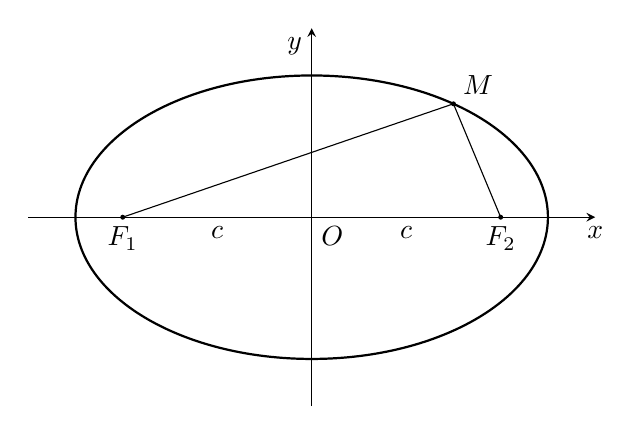
\begin{tikzpicture}[>=stealth, scale=0.6]
		% 1. 绘制坐标轴
		\draw[->] (-6,0) -- (6,0) node[below] {$x$};
		\draw[->] (0,-4) -- (0,4) node[below left] {$y$};
		\node at (0,0) [below right] {$O$};
		
		% 2. 定义椭圆参数(长半轴a=5,短半轴b=3,焦距c=4,满足a²=b²+c²)
		\def\a{5}  % 长半轴
		\def\b{3}  % 短半轴
		\def\c{4}  % 焦距(c = sqrt(a² - b²) = 4)
		
		% 3. 绘制椭圆
		\draw[thick] (0,0) ellipse ({\a} and {\b});
		
		% 4. 标记焦点F1、F2
		\fill (-{\c},0) circle (1.5pt) node[below] {$F_1$};
		\fill ({\c},0) circle (1.5pt) node[below] {$F_2$};
		
		% 5. 标记原点到焦点的距离c
		\draw[dashed] (0,0) -- ({\c},0) node[midway, below] {$c$};
		\draw[dashed] (0,0) -- (-{\c},0) node[midway, below] {$c$};
		
		% 6. 定义椭圆上点M(示例:M(3, 2.4),满足椭圆方程x²/25 + y²/9 = 1)
		\coordinate (M) at (3, 2.4);
		\fill (M) circle (1.5pt) node[above right] {$M$};
		
		% 7. 绘制线段F1M和F2M
		\draw (-{\c},0) -- (M);
		\draw ({\c},0) -- (M);
		
	\end{tikzpicture}
\end{document}
